\section{Problem Definition}
%As we have mentioned, the way Zheng et al. deal with RE is not in the scope of
%both pipeline and joint
%approach, which do not apply two sub-tasks, NER and RC. 
%Here, we define it as a new
%problem, end-to-end RE.

\begin{defn}
  Given a sentence $s$ and a relation type set $\mathcal{R}$, end-to-end
  RE problem is to extract relation triple \{ $e1$, $r$, $e2$ \} by
  predicting entity pair ($e1$, $e2$) and relation type $r$ simultaneously.
\end{defn}

In this paper, following \citet{Zheng2017}, this problem is broken down into two
subproblems: first {\em label} each word in the sentence with a RE tag, and
second {\em reconstruct} the relation triples from the tag sequence.

\subsection{RE tagging problem}
\figref{fig:re-tag} shows the first subproblem.
Our RE tag follows the work of \cite{Zheng2017} and consists of three parts, a relation
type, an entity role and
a relative position. Relation type part is the string of a predefined
relation type such as ``LeaderOf''. The entity role indicate whether it is
$e_1$ or $e_2$ in the relation triple. Here, we use ``1'' or ``2'' 
to make this distinction.  The relative position refers to the same tag used in
traditional NER, i.e., ``B'' (Begin), ``I'' (Inner), ``E'' (End) and ``S''
(Single) to represent the position of tokens in its entity. These three parts
are combined into a full relation tag. For example, in ``LE-1-B'' (for Tim),
``LE'' is the abbreviation of ``LeaderOf'', ``1'' means both ``Tim'' is  $e_1$
of ``LeaderOf'' relation, ``B'' means ``Tim'' is
the beginning of this entity. 
Note that we do not need to encode entity type into RE tagging scheme, 
because we can reconstruct a triple without the knowledge of the type of an
entity.



\begin{figure}[th]
\centering
\includegraphics[width=\columnwidth]{pictures/endre.eps}
\caption{RE Tagging Subproblem \label{fig:re-tag}}
\end{figure}

To solve this problem, we propose a joint RE tagging approach which augments the
work of \cite{Zheng2017} by adding an auxiliary task. To distinguish, we
call \cite{Zheng2017} basic RE tagging approach.



\subsection{Triple reconstruction problem}
Given a relation tag sequence, there may be several ways to
reconstruct the final relation triples. For example, assuming the tag sequence
of sentence $(w_1, w_2, w_3, w_4, w_5)$ is ``LE-1-S, LE-2-S, LE-2-S, LE-1-S,
LE-2-S'', one possibility is to get \{$w_1$, LeaderOf, $w_2$\} by pairing
$w_1$ with $w_2$, and get \{$w_4$, LeaderOf, $w_5$\} by pairing $w_4$ with
$w_5$. Another way to reconstruct the triples is to pair $w_1$ with $w_2$, and
get \{$w_1$, LeaderOf\, $w_2$\}, while pairing $w_4$ with $w_3$ to get \{$w_4$,
LeaderOf, $w_3$\}. This problem is to find the most plausible triple assignment
given a sequence of RE tags. In this paper, we will attempt a number of
heuristics and show their pros and cons.

